\documentclass[11pt]{article}
\usepackage[margin=1in]{geometry}
\usepackage{times}
\usepackage{url}
\usepackage{hyperref}
\usepackage{amsmath,amssymb}
\usepackage{booktabs}
\usepackage{tikz}
\usetikzlibrary{shapes,positioning}
\title{MOTIF: Family-Diverse Multi-Model Development\\
and Runtime-Bound Selection for Continuously Running Systems}
\author{
Keith\thanks{Correspondence: KMesh / COSMOS. Public repositories:
\texttt{https://github.com/keithbbf-gif/cosmos},
\texttt{https://github.com/keithbbf-gif/bts-mesh},
\texttt{https://github.com/keithbbf-gif/cdeck}.}
\and
KMesh / COSMOS
}
\date{September 2026}

\begin{document}
\maketitle

\begin{abstract}
We describe the implementation and operation of COSMOS (Carry-Over
State Mesh Operating System), a resident operating system for AI work
whose primary object is state that survives a session. One service is
the sole authority and the sole writer of an append-only, hash-chained,
service-signed JSONL ledger; workers publish only through a fenced
commit gateway; the system is modified while it remains up. We report
MOTIF, the eight-stage development method used to build COSMOS and to
change it under that constraint: independent architecture, dual-lane
construction with no shared context, different-family critique, and
iterate-to-research. Swiss-cheese occupancy is the design rule for
staffing those stages: a model exposes a hole-set; same-family votes
do not count twice; residual error shrinks with disagreement across
families, not with copies of one API. That a roster of inexpensive,
disagreeing models can beat a single frontier pass on price and task
performance is a hypothesis used to design the loop, not a measured
result. Public GitHub \texttt{created\_at} timestamps are 16, 23, and
24~August~2026. We do not report a controlled benchmark.
\end{abstract}

\section{Introduction}

COSMOS is a running operating system for AI work. It is a modular
monolith: one resident Windows service is the API gateway, scheduler,
lease arbiter with fencing tokens, spend gate, return-watcher, registry
and prober, and the single writer of the ledger. Dashboards, queue
views, and spend totals are rebuildable projections. Large artifacts
live in a content-addressed store; the ledger holds the live pointer.
The object is state that survives a session. Chat is a client.

The development problem this paper reports is not how to wrap another
chat. It is how to modify that resident service \emph{while it stays
up}. A change that would take the system down to install itself is the
wrong change. Keeping the running system alive during self-modification
is a requirement, not a nicety. MOTIF (the default development method
of COSMOS) is the loop used for that class of work: research,
independent architecture, consensus, dual-lane build, different-family
critics, consensus, improve, iterate back to research. None of the
stages is silently skipped. Selection is a runtime-binding gate---a
value only the live tree can emit---not an exit code or a green log.
A claim is not evidence. The report of a change carries the artifact
the live tree emitted, or it carries a refusal.

Software built by a single large language model inherits that model's
blind spots: systematic errors, preferred tools, and a willingness to
invent rather than refuse. Adding a second agent from the same vendor
family typically stacks the same holes. Industry practice often treats
``more agents'' as quality control. If the agents are not diverse in
\emph{family}, they are extra votes for the same mistakes, at extra
cost. A second, independent failure is fabricated compliance: a
pipeline reports success because tests exited zero or a critic produced
agreeable prose. Neither is evidence that the live system now does the
thing.

MOTIF treats plurality as a requirement, not a preference. Dual-lane
build and different-family critics exist to punch \emph{different}
holes. SuperGrok and Grok, for example, are one family: that is three
families of vote, not four. Iterate re-enters research so the
architecture, the primary coder, and the baseline can change. Family
identity is an occupancy rule used in production (shared training
house, tool surface, and failure mode), not a clustering theorem.

We do not report a randomized bake-off. Cheap-plural versus frontier
performance is a hypothesis used to design the loop. Public repository
timestamps and a ratified architecture document exist~\cite{cosmosarch};
a controlled comparison does not, and is not invented here.

\section{System context: COSMOS}

COSMOS (Carry-Over State Mesh Operating System) is a modular-monolith
resident service~\cite{cosmosarch}. One process is the sole authority.
The ledger is append-only JSONL, hash-chained and service-signed; a
corrupt segment refuses rather than repairing in place. Leases carry
fencing tokens so a late writer cannot overwrite a live grant. Workers
(native, DOM, cloud) run in attempt-private workspaces and publish only
through a fenced commit gateway. Projections---queue views, registries,
dashboards, spend totals---are caches. They are never authority.
Internal interfaces are RPC-shaped so a module can later become a
process without breaking the one versioned external API that
dashboards, voice, and phone or desktop clients consume.

DOM is a first-class rail and the preferred rail: it depends on
nothing that can run out (credit, quota, billing, key, consent).
Metered APIs are fallback. The browser path is used when nothing else
works, not only when it is convenient. Roles on the OS (coding, legal,
medical, diligence, physics, IP) share that service; they are not
separate truths.

The fence is the only publish path from an attempt-private workspace
into the live tree. A worker that cannot present a fencing token does
not write. A late holder of an expired lease does not overwrite a live
grant. Fail-closed segments refuse rather than repairing in place;
visible refusals are correct behavior, not faults to route around.
Projections may go green while the ledger has not moved. That is why
the gate is a live emit, not a dashboard.

Occupancy is folded here because it is how the artifact stays up, not a
second argument. Orchestration is not coding. One chief coder writes
the live tree at a time; adversarial builders propose; workers publish
through the fence. If the orchestrator also holds the only wrench, the
system will eventually ship a plausible lie. A change that would take
the system down to install itself is the wrong change. Same-family
votes do not count twice: Grok and SuperGrok share a house, a tool
surface, and a failure mode, so they are one family of vote.

Self-modification under that occupancy is the systems claim. MOTIF
stages run against the live service; builders land on branches; the
chief coder is the only writer of the running tree; the fence is the
only publish path. The architecture was ratified on the same day the
public \texttt{cosmos} repository was created. The service was not
taken down to install the method that now modifies it.

A predecessor mesh (BTS-MESH) operated this class of work in July 2026,
attested by dated local run records. Public GitHub timestamps:
\texttt{bts-mesh} created 16~August~2026;
\texttt{cosmos} created 23~August~2026 (ratification day);
\texttt{cdeck} created 24~August~2026. July operation and August public
dates are not the same fact.

\section{Swiss cheese}

Let $H(m)$ be the hole-set of model $m$ (error classes, unseen tools,
fabrication modes). One model exposes the work to $H(m_1)$. Two models
of one family satisfy $H(m_1)\approx H(m_2)$. Two models of different
families expose $H(m_1)\cap H(m_2)$, which is smaller if the families
actually disagree. For $N$ models, residual holes shrink with genuine
disagreement, not with $N$ copies of one API.

\begin{figure}[h]
\centering
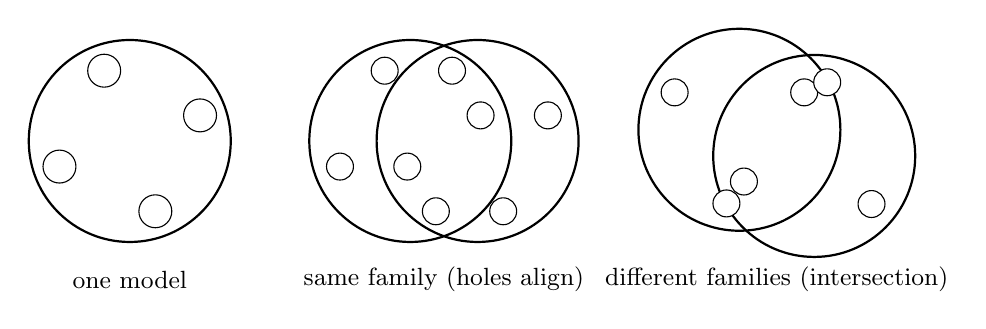
\begin{tikzpicture}[scale=0.95]
  \draw[thick] (0,0) circle (1.35);
  \node at (0,-1.85) {\small one model};
  \foreach \a in {20,110,200,290} {
    \fill[white] ({1.0*cos(\a)},{1.0*sin(\a)}) circle (0.22);
    \draw ({1.0*cos(\a)},{1.0*sin(\a)}) circle (0.22);
  }
  \begin{scope}[shift={(4.1,0)}]
    \draw[thick] (-0.35,0) circle (1.35);
    \draw[thick] (0.55,0) circle (1.35);
    \node at (0.1,-1.85) {\small same family (holes align)};
    \foreach \a in {20,110,200,290} {
      \fill[white] ({1.0*cos(\a)-0.35},{1.0*sin(\a)}) circle (0.18);
      \draw ({1.0*cos(\a)-0.35},{1.0*sin(\a)}) circle (0.18);
      \fill[white] ({1.0*cos(\a)+0.55},{1.0*sin(\a)}) circle (0.18);
      \draw ({1.0*cos(\a)+0.55},{1.0*sin(\a)}) circle (0.18);
    }
  \end{scope}
  \begin{scope}[shift={(8.6,0)}]
    \draw[thick] (-0.45,0.15) circle (1.35);
    \draw[thick] (0.55,-0.2) circle (1.35);
    \node at (0.05,-1.85) {\small different families (intersection)};
    \foreach \a in {30,150,260} {
      \fill[white] ({1.0*cos(\a)-0.45},{1.0*sin(\a)+0.15}) circle (0.18);
      \draw ({1.0*cos(\a)-0.45},{1.0*sin(\a)+0.15}) circle (0.18);
    }
    \foreach \a in {80,200,320} {
      \fill[white] ({1.0*cos(\a)+0.55},{1.0*sin(\a)-0.2}) circle (0.18);
      \draw ({1.0*cos(\a)+0.55},{1.0*sin(\a)-0.2}) circle (0.18);
    }
  \end{scope}
\end{tikzpicture}
\caption{Hole-sets. Same-family slices leave holes aligned.
Different-family slices shrink the residual intersection. The drawing
is schematic, not a measured Venn of any vendor pair.}
\end{figure}

This picture is an analogy to Reason's accident-causation
model~\cite{reason1990,reason2000}, not that model claimed as ours.
We borrow slices with holes and apply them to model families.

The same pattern is forty years old in software fault tolerance.
$N$-version programming proposed independently written versions as
coverage~\cite{avizienis}. Knight and Leveson showed that independently
written versions \emph{do not} fail independently~\cite{knightleveson}.
Aligned holes across same-family language-model slices are that result
in the present tooling.

\textbf{Claim (operational).} Method power increases with (i)~axis of
difference across models (vendor, training mixture,
tool/code/reason/search, cost tier) and (ii)~the number of such models.
That a roster of inexpensive, disagreeing models can beat a single
frontier model on price and task performance is a hypothesis used to
design MOTIF, not a result reported here. A monoculture of the
frontier model is, on that hypothesis, the expensive way to keep the
same holes.

\section{The MOTIF loop}

Stages, in order; none silently skipped. A third party can
re-implement the method at this grain (stages plus occupancy), not as
a survey of the field.

\begin{enumerate}
\item \textbf{Research.} Returns on disk before build. Prefer rails
that cannot run out of credit (DOM/browser first; metered APIs
second). Every URL and DOI is verified.
\item \textbf{Architecture.} Rubric first. Independent designs. No
peeking. Same-family architects are not two designs.
\item \textbf{Consensus.} Converge, or mark contested (both positions,
one line to the human). No third model resolves.
\item \textbf{Build.} Dual lane, no shared context. Two builders, not
builder-plus-checker. Each spike must run. Code lands on branches;
the live tree has one writer.
\item \textbf{Critics.} Different family. Judge against \emph{what was
decided}, not against surface prettiness. Net complexity should fall
as capability rises.
\item \textbf{Consensus.} Reconcile critiques. Prior versions are
baselines; a regression is a finding.
\item \textbf{Improve.} Apply; subtract as well as add.
\item \textbf{Iterate.} Return to \textbf{research}, not to critics. A
5--8 loop polishes. A 1--8 loop can replace the architecture, the
primary coder, and the baseline.
\end{enumerate}

Dual-lane isolation is the implemented countermeasure to
shared-context pollution~\cite{talkcheap}: a weak lane that can talk
to a strong lane mid-pass will often move a correct answer to an
incorrect one. The lanes do not share a transcript. Each must produce
a running spike from the same decision. Compare is a later consensus
step, not a silent merge by a third model. Different-family critics
are the implemented countermeasure to majority collapse among similar
models~\cite{estornell,debatevote,moreagents}. They judge against
\emph{what was decided}, not against house style. Iterate-to-research
is how the loop remains able to replace the thing already built when a
new model, fact, or need arrives. A critics-only loop (stages 5--8)
can only polish.

The gate is runtime binding: a value only the live tree can emit.
Exit codes and green logs are not evidence. A claim is not evidence.

\section{Related work}

Multi-agent debate as a method for factuality and reasoning is due to
Du et al.~\cite{debate}. Liang et al.\ give a multi-agent debate
(MAD) framework in which agents argue tit-for-tat under a
judge~\cite{mad}. Irving, Christiano, and Amodei framed two agents
arguing for a judge as a safety mechanism~\cite{irving}.
Mixture-of-Agents aggregates generations across a layered roster of
models~\cite{moa}. Self-consistency samples diverse chains from
\emph{one} model~\cite{selfcons}; it is coverage of a single hole-set,
not of a family axis.

Role-playing and coding crews orchestrate agents around a shared
transcript: CAMEL~\cite{camel}, AutoGen~\cite{autogen},
ChatDev~\cite{chatdev}, MetaGPT~\cite{metagpt}. Workflow products
(LangGraph, n8n, Dify, CrewAI) add graphs, interrupts, and studios;
they are named as products, not as papers.

Two clusters of results bear directly on occupancy. First, similar
models do not supply independent coverage. Estornell and Liu show that
similar-model debate collapses to majority---a ``tyranny of the
majority'' when the majority encodes a shared
misconception~\cite{estornell}. Choi, Zhu, and Li find that majority
voting often accounts for most of the gain attributed to
debate~\cite{debatevote}. Li et al.\ show that sampling-and-voting
scales with the number of agents, often instantiated from the
\emph{same} model~\cite{moreagents}. Together those results block the
naive claim that $N$ copies equal coverage. Knight and Leveson is the
classical form of the same block~\cite{knightleveson}.

Second, naive mixing can pollute. Wynn, Satija, and Hadfield show that
debate among weak and strong agents that \emph{share context} can move
a correct answer to an incorrect one when agents prefer agreement over
resistance to flawed reasoning~\cite{talkcheap}. Zhu et al.\ report
that diversity of initial viewpoints helps debate only when it is real
diversity, not noise injected into a shared channel~\cite{demystify}.

MOTIF does not replace those lines of work. It implements constraints
that respond to them: family-axis plurality rather than $N$ clones of
one API; dual-lane build without shared context; iterate-to-research
rather than critics-only polish; runtime-binding versus green-log; one
live-tree writer so the system stays up while it is modified. We did
not invent the failure modes. Avizienis stated the $N$-version hope;
Knight and Leveson measured the independence assumption and found it
false; Estornell and Liu, Choi et al., and Li et al.\ measured the
language-model form of extra votes; Wynn, Satija, and Hadfield measured
shared-context pollution. MOTIF's occupancy rules are those
measurements turned into seats: who may write, who may not share a
transcript, which products count as one family, and what the live tree
must emit before a change is done.

\section{Evaluation boundary}

No randomized benchmark is reported in this manuscript. Cost and task
performance of inexpensive plural rosters versus a frontier singleton
is an operational hypothesis used to design the loop, to be measured
per task; it is not a result. Family identity is an occupancy rule in
production, not a clustering theorem and not a market partition.
Public GitHub is provenance of \texttt{created\_at} dates, not a dump
of the live ledger, not a first-commit date inside each repository
(those were not fetched), and not the runtime-binding gate. The method
is re-implementable at the grain of stages plus occupancy, not as a
survey of debate, crews, or $N$-version programming. This manuscript
is not a patent filing.

\section{Conclusion}

COSMOS is implemented and operated: one writer, a fail-closed ledger,
a fenced commit gateway, DOM-first rails, and state that survives a
session. MOTIF is the method used to modify that system while it stays
up. Occupancy---family-axis plurality, dual-lane isolation,
iterate-to-research, runtime-binding---responds to known failure modes
in debate, $N$-version programming, and shared-context crews. A third
party can re-implement the stages and the occupancy rules at the level
described. We do not report a controlled bake-off.

\section*{Use of language tools}

This manuscript was prepared with assistance from large language model
tools under the author's direction. The author takes full
responsibility for its contents, including citations. Generative tools
are not authors.

\begin{thebibliography}{99}

\bibitem{debate}
Y.~Du, S.~Li, A.~Torralba, J.~B.~Tenenbaum, and I.~Mordatch,
``Improving factuality and reasoning in language models through multiagent debate,''
in \emph{Proc.\ ICML}, 2024.
Also arXiv:2305.14325.

\bibitem{mad}
T.~Liang, Z.~He, W.~Jiao, X.~Wang, Y.~Wang, R.~Wang, Y.~Yang, S.~Shi, and Z.~Tu,
``Encouraging divergent thinking in large language models through multi-agent debate,''
in \emph{Proc.\ EMNLP}, 2024.
Also arXiv:2305.19118.

\bibitem{moa}
J.~Wang, J.~Wang, B.~Athiwaratkun, C.~Zhang, and J.~Zou,
``Mixture-of-Agents enhances large language model capabilities,''
arXiv:2406.04692, 2024.
ICLR 2025 Spotlight (OpenReview \texttt{h0ZfDIrj7T}).

\bibitem{irving}
G.~Irving, P.~Christiano, and D.~Amodei,
``AI safety via debate,''
arXiv:1805.00899, 2018.

\bibitem{selfcons}
X.~Wang, J.~Wei, D.~Schuurmans, Q.~Le, E.~Chi, S.~Narang, A.~Chowdhery, and D.~Zhou,
``Self-consistency improves chain of thought reasoning in language models,''
in \emph{Proc.\ ICLR}, 2023.
Also arXiv:2203.11171.

\bibitem{debatevote}
H.~K.~Choi, X.~Zhu, and S.~Li,
``Debate or vote: Which yields better decisions in multi-agent large language models?''
arXiv:2508.17536, 2025. NeurIPS 2025 Spotlight.

\bibitem{talkcheap}
A.~Wynn, H.~Satija, and G.~Hadfield,
``Talk isn't always cheap: Understanding failure modes in multi-agent debate,''
arXiv:2509.05396, 2025. ICML MAS Workshop 2025.

\bibitem{demystify}
X.~Zhu, C.~Zhang, Y.~Chi, T.~Stafford, N.~Collier, and A.~Vlachos,
``Demystifying multi-agent debate: The role of confidence and diversity,''
arXiv:2601.19921, 2026.

\bibitem{estornell}
A.~Estornell and Y.~Liu,
``Multi-LLM debate: Framework, principals, and interventions,''
in \emph{Adv.\ Neural Inf.\ Process.\ Syst.}, vol.~37, 2024.

\bibitem{moreagents}
J.~Li, Q.~Zhang, Y.~Yu, Q.~Fu, and D.~Ye,
``More agents is all you need,''
arXiv:2402.05120, 2024. TMLR.

\bibitem{autogen}
Q.~Wu, G.~Bansal, J.~Zhang, Y.~Wu, B.~Li, E.~Zhu, L.~Jiang, X.~Zhang, S.~Zhang, J.~Liu, A.~H.~Awadallah, R.~W.~White, D.~Burger, and C.~Wang,
``AutoGen: Enabling next-gen LLM applications via multi-agent conversation,''
arXiv:2308.08155, 2023.

\bibitem{chatdev}
C.~Qian, W.~Liu, H.~Liu, N.~Chen, Y.~Dang, J.~Li, C.~Yang, W.~Chen, Y.~Su, X.~Cong, J.~Xu, D.~Li, Z.~Liu, and M.~Sun,
``ChatDev: Communicative agents for software development,''
in \emph{Proc.\ ACL}, 2024.
Also arXiv:2307.07924.

\bibitem{metagpt}
S.~Hong, M.~Zhuge, J.~Chen, X.~Zheng, Y.~Cheng, C.~Zhang, J.~Wang, Z.~Wang, S.~K.~S.~Yau, Z.~Lin, L.~Zhou, C.~Ran, L.~Xiao, C.~Wu, and J.~Schmidhuber,
``MetaGPT: Meta programming for a multi-agent collaborative framework,''
arXiv:2308.00352, 2023.

\bibitem{camel}
G.~Li, H.~A.~A.~K.~Hammoud, H.~Itani, D.~Khizbullin, and B.~Ghanem,
``CAMEL: Communicative agents for `mind' exploration of large language model society,''
in \emph{Adv.\ Neural Inf.\ Process.\ Syst.}, 2023.
Also arXiv:2303.17760.

\bibitem{avizienis}
A.~Avizienis,
``The $N$-version approach to fault-tolerant software,''
\emph{IEEE Trans.\ Softw.\ Eng.}, vol.~SE-11, no.~12, pp.~1491--1501, 1985.

\bibitem{knightleveson}
J.~C.~Knight and N.~G.~Leveson,
``An experimental evaluation of the assumption of independence in multiversion programming,''
\emph{IEEE Trans.\ Softw.\ Eng.}, vol.~SE-12, no.~1, pp.~96--109, 1986.

\bibitem{reason1990}
J.~Reason,
\emph{Human Error}.
Cambridge University Press, 1990.

\bibitem{reason2000}
J.~Reason,
``Human error: models and management,''
\emph{BMJ}, vol.~320, pp.~768--770, 2000.
PMC1070929.

\bibitem{cosmosarch}
KMesh,
``COSMOS final architecture'' (ratified 23~August~2026)
and MOTIF method note (encoded 25~August~2026).
Public tree: \url{https://github.com/keithbbf-gif/cosmos}.
Not a peer-reviewed item.

\end{thebibliography}

\end{document}
